% This is "sig-alternate.tex" V2.1 April 2013
% This file should be compiled with V2.5 of "sig-alternate.cls" May 2012
%
% This example file demonstrates the use of the 'sig-alternate.cls'
% V2.5 LaTeX2e document class file. It is for those submitting
% articles to ACM Conference Proceedings WHO DO NOT WISH TO
% STRICTLY ADHERE TO THE SIGS (PUBS-BOARD-ENDORSED) STYLE.
% The 'sig-alternate.cls' file will produce a similar-looking,
% albeit, 'tighter' paper resulting in, invariably, fewer pages.
%
% ----------------------------------------------------------------------------------------------------------------
% This .tex file (and associated .cls V2.5) produces:
%       1) The Permission Statement
%       2) The Conference (location) Info information
%       3) The Copyright Line with ACM data
%       4) NO page numbers
%
% as against the acm_proc_article-sp.cls file which
% DOES NOT produce 1) thru' 3) above.
%
% Using 'sig-alternate.cls' you have control, however, from within
% the source .tex file, over both the CopyrightYear
% (defaulted to 200X) and the ACM Copyright Data
% (defaulted to X-XXXXX-XX-X/XX/XX).
% e.g.
% \CopyrightYear{2007} will cause 2007 to appear in the copyright line.
% \crdata{0-12345-67-8/90/12} will cause 0-12345-67-8/90/12 to appear in the copyright line.
%
% ---------------------------------------------------------------------------------------------------------------
% This .tex source is an example which *does* use
% the .bib file (from which the .bbl file % is produced).
% REMEMBER HOWEVER: After having produced the .bbl file,
% and prior to final submission, you *NEED* to 'insert'
% your .bbl file into your source .tex file so as to provide
% ONE 'self-contained' source file.
%
% ================= IF YOU HAVE QUESTIONS =======================
% Questions regarding the SIGS styles, SIGS policies and
% procedures, Conferences etc. should be sent to
% Adrienne Griscti (griscti@acm.org)
%
% Technical questions _only_ to
% Gerald Murray (murray@hq.acm.org)
% ===============================================================
%
% For tracking purposes - this is V2.0 - May 2012

\documentclass{sig-alternate-05-2015}

\usepackage[utf8]{inputenc}
\usepackage[ngerman]{babel}

\begin{document}

% Copyright
%\setcopyright{acmcopyright}
%\setcopyright{acmlicensed}
%\setcopyright{rightsretained}
%\setcopyright{usgov}
%\setcopyright{usgovmixed}
%\setcopyright{cagov}
%\setcopyright{cagovmixed}


% DOI
%\doi{10.475/123_4}

% ISBN
%\isbn{123-4567-24-567/08/06}

%Conference
%\conferenceinfo{PLDI '13}{June 16--19, 2013, Seattle, WA, USA}

%\acmPrice{\$15.00}

%
% --- Author Metadata here ---
%\conferenceinfo{WOODSTOCK}{'97 El Paso, Texas USA}
%\CopyrightYear{2007} % Allows default copyright year (20XX) to be over-ridden - IF NEED BE.
%\crdata{0-12345-67-8/90/01}  % Allows default copyright data (0-89791-88-6/97/05) to be over-ridden - IF NEED BE.
% --- End of Author Metadata ---

\title{Alternate {\ttlit ACM} SIG Proceedings Paper in LaTeX
Format\titlenote{(Produces the permission block, and
copyright information). For use with
SIG-ALTERNATE.CLS. Supported by ACM.}}
\subtitle{[Extended Abstract]
\titlenote{A full version of this paper is available as
\textit{Author's Guide to Preparing ACM SIG Proceedings Using
\LaTeX$2_\epsilon$\ and BibTeX} at
\texttt{www.acm.org/eaddress.htm}}}
%
% You need the command \numberofauthors to handle the 'placement
% and alignment' of the authors beneath the title.
%
% For aesthetic reasons, we recommend 'three authors at a time'
% i.e. three 'name/affiliation blocks' be placed beneath the title.
%
% NOTE: You are NOT restricted in how many 'rows' of
% "name/affiliations" may appear. We just ask that you restrict
% the number of 'columns' to three.
%
% Because of the available 'opening page real-estate'
% we ask you to refrain from putting more than six authors
% (two rows with three columns) beneath the article title.
% More than six makes the first-page appear very cluttered indeed.
%
% Use the \alignauthor commands to handle the names
% and affiliations for an 'aesthetic maximum' of six authors.
% Add names, affiliations, addresses for
% the seventh etc. author(s) as the argument for the
% \additionalauthors command.
% These 'additional authors' will be output/set for you
% without further effort on your part as the last section in
% the body of your article BEFORE References or any Appendices.

\numberofauthors{8} %  in this sample file, there are a *total*
% of EIGHT authors. SIX appear on the 'first-page' (for formatting
% reasons) and the remaining two appear in the \additionalauthors section.
%
\author{
% You can go ahead and credit any number of authors here,
% e.g. one 'row of three' or two rows (consisting of one row of three
% and a second row of one, two or three).
%
% The command \alignauthor (no curly braces needed) should
% precede each author name, affiliation/snail-mail address and
% e-mail address. Additionally, tag each line of
% affiliation/address with \affaddr, and tag the
% e-mail address with \email.
%
% 1st. author
\alignauthor
Martin Root\\
       \email{st100506@stud.uni-stuttgart.de}
% 2nd. author
\alignauthor
Christian Bäumlisberger\\
       \email{st114381@stud.uni-stuttgart.de}
% 3rd. author
\alignauthor
Velihan Bulut\\
       \email{st103204@stud.uni-stuttgart.de}
\and
% 4th. author
\alignauthor Lawrence P. Leipuner\\
       \affaddr{Brookhaven Laboratories}\\
       \affaddr{Brookhaven National Lab}\\
       \affaddr{P.O. Box 5000}\\
       \email{lleipuner@researchlabs.org}
% 5th. author
\alignauthor Sean Fogarty\\
       \affaddr{NASA Ames Research Center}\\
       \affaddr{Moffett Field}\\
       \affaddr{California 94035}\\
       \email{fogartys@amesres.org}
% 6th. author
\alignauthor Charles Palmer\\
       \affaddr{Palmer Research Laboratories}\\
       \affaddr{8600 Datapoint Drive}\\
       \affaddr{San Antonio, Texas 78229}\\
       \email{cpalmer@prl.com}
}
% There's nothing stopping you putting the seventh, eighth, etc.
% author on the opening page (as the 'third row') but we ask,
% for aesthetic reasons that you place these 'additional authors'
% in the \additional authors block, viz.
\additionalauthors{Additional authors: John Smith (The Th{\o}rv{\"a}ld Group,
email: {\texttt{jsmith@affiliation.org}}) and Julius P.~Kumquat
(The Kumquat Consortium, email: {\texttt{jpkumquat@consortium.net}}).}
\date{30 July 1999}
% Just remember to make sure that the TOTAL number of authors
% is the number that will appear on the first page PLUS the
% number that will appear in the \additionalauthors section.

\maketitle
\begin{abstract}
This paper provides a sample of a \LaTeX\ document which conforms,
somewhat loosely, to the formatting guidelines for
ACM SIG Proceedings. It is an {\em alternate} style which produces
a {\em tighter-looking} paper and was designed in response to
concerns expressed, by authors, over page-budgets.
It complements the document \textit{Author's (Alternate) Guide to
Preparing ACM SIG Proceedings Using \LaTeX$2_\epsilon$\ and Bib\TeX}.
This source file has been written with the intention of being
compiled under \LaTeX$2_\epsilon$\ and BibTeX.

The developers have tried to include every imaginable sort
of ``bells and whistles", such as a subtitle, footnotes on
title, subtitle and authors, as well as in the text, and
every optional component (e.g. Acknowledgments, Additional
Authors, Appendices), not to mention examples of
equations, theorems, tables and figures.

To make best use of this sample document, run it through \LaTeX\
and BibTeX, and compare this source code with the printed
output produced by the dvi file. A compiled PDF version
is available on the web page to help you with the
`look and feel'.
\end{abstract}


%
% The code below should be generated by the tool at
% http://dl.acm.org/ccs.cfm
% Please copy and paste the code instead of the example below. 
%
%\begin{CCSXML}
%<ccs2012>
% <concept>
%  <concept_id>10010520.10010553.10010562</concept_id>
%  <concept_desc>Computer systems organization~Embedded systems</concept_desc>
%  <concept_significance>500</concept_significance>
% </concept>
% <concept>
%  <concept_id>10010520.10010575.10010755</concept_id>
%  <concept_desc>Computer systems organization~Redundancy</concept_desc>
%  <concept_significance>300</concept_significance>
% </concept>
% <concept>
%  <concept_id>10010520.10010553.10010554</concept_id>
%  <concept_desc>Computer systems organization~Robotics</concept_desc>
%  <concept_significance>100</concept_significance>
% </concept>
% <concept>
%  <concept_id>10003033.10003083.10003095</concept_id>
%  <concept_desc>Networks~Network reliability</concept_desc>
%  <concept_significance>100</concept_significance>
% </concept>
%</ccs2012>  
%\end{CCSXML}

%\ccsdesc[500]{Computer systems organization~Embedded systems}
%\ccsdesc[300]{Computer systems organization~Redundancy}
%\ccsdesc{Computer systems organization~Robotics}
%\ccsdesc[100]{Networks~Network reliability}


%
% End generated code
%

%
%  Use this command to print the description
%
\printccsdesc

% We no longer use \terms command
%\terms{Theory}

\keywords{ACM proceedings; \LaTeX; text tagging}

\section{Introduction}

\section{Grundlagen}

In diesem Kapitel werden die Grundlagen dieser Arbeit beschrieben. Dazu gehören unter anderem einige technischen Details über KDE, Wissenswertes über die Versionshistorie, sowie der aktuelle Stand des Projekts.

\subsection{Übersicht}
In der heutigen Computerwelt ist die Interaktion zwischen Mensch und Computer ohne eine graphische Benutzeroberfläche nahezu undenkbar. Daher gibt es eine große Auswahl an unterschiedlichen Betriebssystemen, die auch unterschiedliche Benutzeroberflächen haben. Eines dieser graphischen Benutzeroberflächen ist KDE.

\begin{figure}[h]
	\centering
	
\includegraphics[width=0.7\linewidth]{images/KDE_logo.png}
	\caption{Aktuelles offizielles KDE Logo. \cite{kdelogo}}
	\label{fig:kdelogo}
\end{figure}

KDE stand ursprünglich für \textit{Kool Desktop Environment} und steht heute für \textit{K Desktop Environment}, zu deutsch \textit{K Arbeitsumgebung}, wobei das \textit{K} keine bestimmte Bedeutung mehr hat, sondern als eine Art Markenzeichen von KDE ist. Es handelt sich dabei um eine graphische Arbeitsumgebung für UNIX-Betriebssysteme. Es besteht aus einer Reihe von kleinen Programmen, einem Fenstermanager, einem Dateimanager und einigen Hilfsprogrammen. Das Ziel von KDE ist es, die Verwendung von UNIX-basierten Betriebssystemen zu vereinfachen. \cite{TUChemnitzKDE}. Bild \ref{fig:kdelogo} zeigt das aktuelle offizielle KDE Logo.

\subsection{Versionshistorie}
Das KDE Projekt wurde am 14. Oktober 1996 von Matthias Ettrich begonnen. Sowohl der Name also auch der Funktionsumfang des Projekts orientierte sich an der proprietäre Desktop-Umgebung CDE (\textit{Common Desktop Environment}). KDE setzte von Beginn an auf die Programmiersprache C++ und auf die umfangreiche Oberflächenbibliothek \textit{Qt}.

Die KDE-Komponenten wurden ziemlich unkoordiniert entwickelt, weshalb es keine einheitlichen Alpha-Version gab. Etwa ein Jahr nach der Gründung von KDE erschien am 20. Oktober 1997 die erste Beta-Version. Nach drei weiteren Beta-Versionen wurde am 12. Juli 1998 die Version 1.0 von KDE präsentiert und veröffentlicht. Abbildung \ref{fig:kdeversion1} zeigt einen Standbild der Benutzeroberfläche von K Desktop Environments Version 1.0. Trotz einiger Kritik wegen der unfreien Bibliothek Qt konnte sie sich durchsetzen und fand seinen weg in einige Linux-Distributionen. \cite{kdeversion1}

\begin{figure}[h]
	\centering
	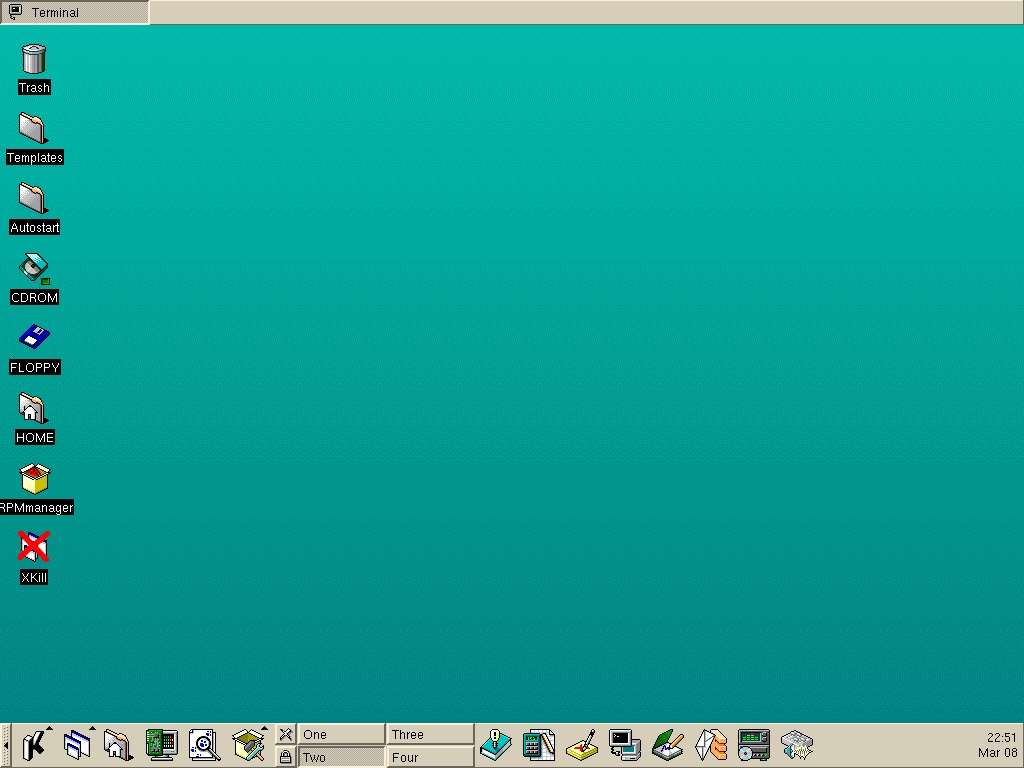
\includegraphics[width=\linewidth]{images/KDE_1.png}
	\caption{KDE Version 1.0 \cite{kdeversionenwiki}}
	\label{fig:kdeversion1}
\end{figure}

In den folgenden beiden Jahren wurde KDE durch zahlreiche Verbesserungen in einigen Punkten den Wünschen von Nutzern angepasst und auf die Version 1.1 gebracht. Durch eine neue Version der Oberflächenbibliothek Qt stand KDE vor vielen Verbesserungen, weshalb man sich entschied, die Verbesserungen nicht in die erste Generation von KDE aufzunehmen. Dieser Versionssprung wurde dazu genutzt die unkoordinierte Entwicklung und die Infrastruktur des Projekts zu überarbeiten. Bis zu Veröffentlichung wurde auch Qt unter die Lizenz GPL 2.0 gestellt, wodurch der Lizenzkonflikt zwischen den Lizenzen von KDE und Qt behoben wurde.

Die stabile Version von K Desktop Environments 2.0 wurde schließlich am 23. Oktober 2000 veröffentlicht. Abgesehen von den der besseren Infrastruktur wurde diese Version nun mit der freien Bibliothek Qt 2.2 veröffentlicht. Des Weitere erntete auch \textit{Konqueror}, der neue KDE-Dateimanager und -Webbrowser, viel positive Kritik. Andere Websbrowser waren zu dieser Zeit sehr unstabil oder nicht fertiggestellt. Abbildung \ref{fig:kdeversion2} zeigt die Benutzeroberfläche von K Desktop Environments 2 und den Webbrowser Konqueror. Durch KDE 2.0 konnte sich das Unternehmen als feste Institution unter den X11-Oberflächen durchsetzen.

\begin{figure}[h]
	\centering
	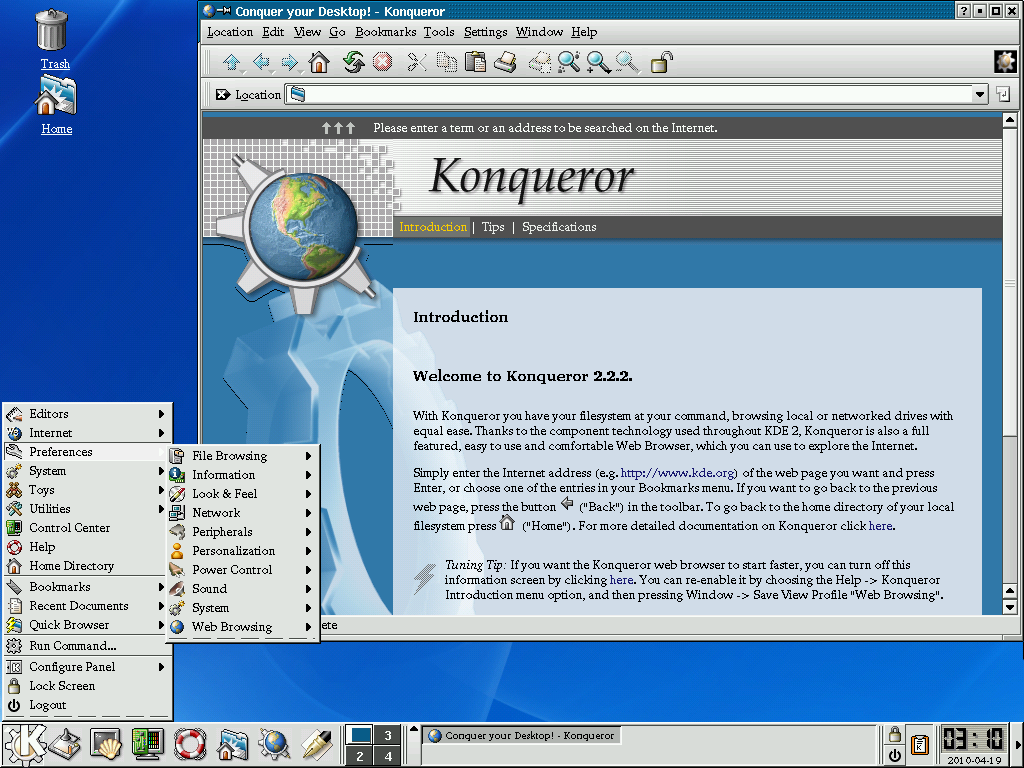
\includegraphics[width=\linewidth]{images/KDE_222.png}
	\caption{KDE Version 2.2.2 \cite{kdeversionenwiki}}
	\label{fig:kdeversion2}
\end{figure}

Nach zahlreichen Verbesserungen und zwei weiteren Veröffentlichungen von KDE in der zweiten Generation erschien am 3. April 2002 die Version 3.0. Diese und die darauffolgenden Versionen der 3. Generation brachten viele Neuerungen. Dazu zählten beispielsweise das \textit{Desktop Sharing Framework}, wodurch KDE-Desktops von entfernten Rechner verwendet werden konnten, \textit{Tabbed Browsing} in Konqueror und einen integrierten \textit{Personal Information Manager} namens \textit{Kontact}, das in einer Anwendung nützliche Funktionen wie E-Mail, Adressbuch, Kalender, Terminplaner, Newsreader, Wetteranzeige, Geburtstagserinnerung, Notizblock und Aufgabenliste kombinierte. Außerdem wurde der Benutzeroberfläche durch überarbeitete Icons und (in einigen Bereichen) durch neuem Design ein modernes Aussehen verliehen. In Abbildung \ref{fig:kdeversion3} ist K Desktop Environments in der Version 3.5 zu sehen.

\begin{figure}[h]
	\centering
	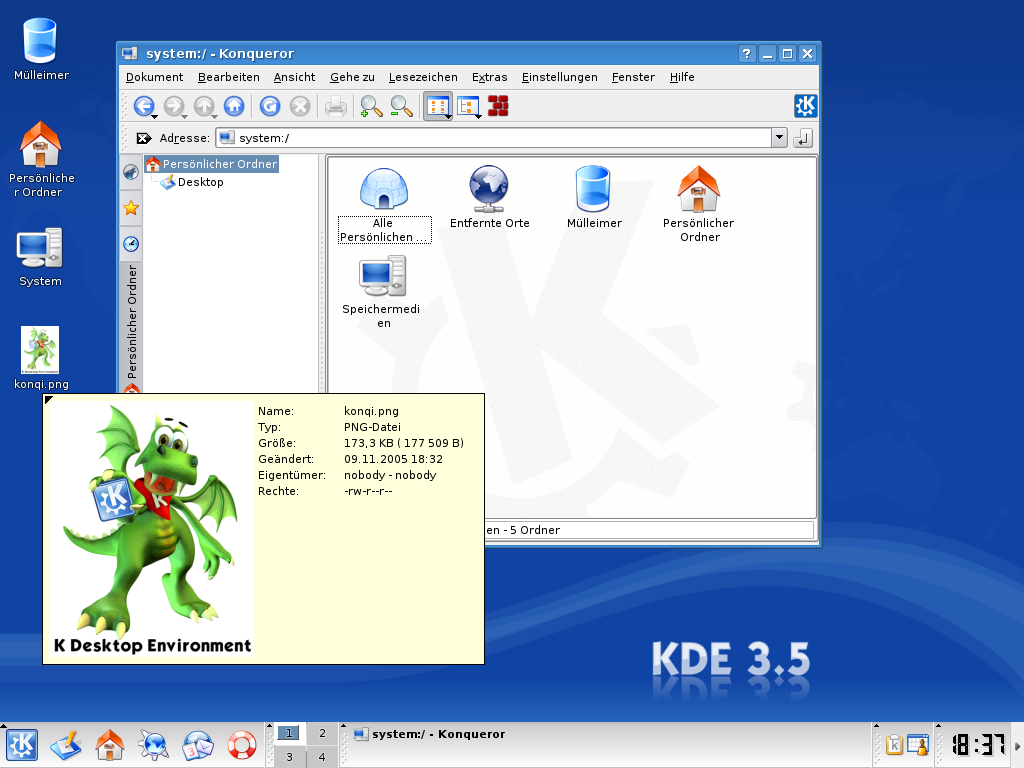
\includegraphics[width=\linewidth]{images/KDE_35.png}
	\caption{KDE Version 3.5 \cite{kdeversionenwiki}}
	\label{fig:kdeversion3}
\end{figure}

In der darauffolgenden Version wurde die Ausformulierung K Desktop Environments nicht mehr verwendet und es erschien am  11. Januar 2008 KDE 4.






\section{KDE Requirements Engineering}

Der folgende Teil beschreibt das Requirements Engineering bei dem Open Source
Projekt KDE. Ein Großteil der Informationen wurde der offiziellen
deutschsprachigen Website von KDE entnommen\cite{1}. 
%Quelle:https://de.kde.org/

\subsection{Requirement Engineering}
Requirements Engineering umfasst das Ermitteln, Analysieren, Spezifizieren und
Validieren aller Eigenschaften und Rahmenbedingungen eines Softwaresystems, die
über seinen gesamten Lebenszyklus gewünscht werden bzw. relevant sind\cite{2}.  
%Quelle:http://www.enzyklopaedie-der-wirtschaftsinformatik.de/lexikon/is-management/Systementwicklung/Hauptaktivitaten-der-Systementwicklung/Problemanalyse-/Requirements-Engineering/index.html

\subsection{Requirement Engineering in Open Source projekten}
Requirement Engineering bei Open Source Projekten unterscheidet sich von dem
gewöhnlicher Projekte(wie z.B. bei Firmen die als Dienstleister Software
entwickeln). Normalerweise werden die Anforderungen vom Kunden entgegen genommen
und zusammen mit dem Ersteller der Software zu realistischen und
aufgabenorientierten Requierements umformuliert. Doch bei Open Source Projekten
gilt es bestimmte Ziele zu erfüllen, wie das Endprodukt ausehen soll, dann
werden Requirements von der Community gegeben und von den Entwicklern erstellt.

%Quelle:

\subsection{Quellen für Requirements bei KDE}
Das Sammeln von Requirements bei KDE erfolgt über Benutzer Feedback,
Fehlerrückmeldungen und wirtschaftlichen Interessen. Feedback und Fehler werden
auf der Website über eine Adresse angenommen\cite{3}.
%http://bugs.kde.org 
%über das sammeln von requirements wegen wirtschaftlichen Interessen wurde
%nichts weiter? angegegben
% Quelle:https://techbase.kde.org/Development/Software_Engineering_Framework#Requirements_Gathering

\subsection{Dokumentation von KDE}
Die Dokumentation von KDE wird mit dem Produkt selbst ausgeliefert und dient
auch als hilfe Datei. Deswegen ist sie mehr als Handbuch bzw. als Hilfestellung
gedacht und weniger zum formulieren, festhalten oder entnehmen von Requirements.
Als Beispiel wird einem gezeigt wie man die Lautstärke für Ausgabegeräte
einstellt aber nicht welche Anforderungen an den Lautstärke Regler gestellt
wurden\cite{4}.

%Quelle:https://docs.kde.org/index.php?language=de&package=kdemultimedia
\subsection{Umgang mit Requirements bei KDE}
Die Arbeit an KDE verläuft ähnlich zu der bei Linux. Eine Aufgabe wird in
Teilaufgaben aufgeteilt, dann werden verantwortliche für diese Teilaufgaben
gesucht und denen die Teilaufgabe übertragen. Wodurch diese als Ansprechpartner
und Verantwortlicher dafür dienen. Als Beispiel kann man in folgendem Bild
KDEgames sehen.
%
\begin{figure}[h]
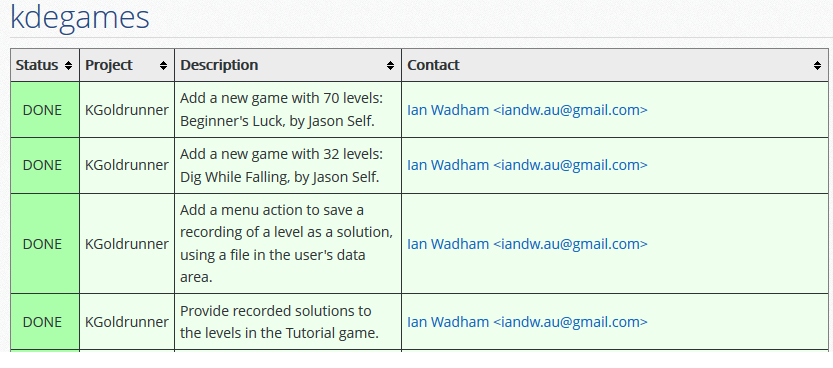
\includegraphics[width=\columnwidth]{images/KDE_games.png}
\caption{KDEgames\cite{5}}
\end{figure}
%Bild KDE Games
Das Bild zeigt einen Ausschnitt einer Tabelle die der Quelle, der KDE
Website entnommen wurde\cite{5}.
%Quelle:https://techbase.kde.org/Schedules/Applications/15.12_Feature_Plan
Die Tabelle hat vier Spalten. Die Erste zeigt den Status der Aufgabe an, DONE
IN PROGRESS oder TODO. Die zweite zeigt den Namen des Projekts. Die Dritte eine Beschreibung des Projekts und die vierte den Verantwortlichen für das Projekt.\\
Dadurch wird die Bearbeitung der einzelnen Projekte dokumentiert.

Besprochen werden die Requirements und andere Aufgabenspezifische teile über Mailinglisten. Damit werden Diskussionen und Absprachen durchgeführt.
Diese kann man ebenfalls über die Website einsehen, um einen Einblick in den
Verlauf eines Projekts zu erhalten.

Zusätzlich werden noch Requirements an bestimmte Teile des Produkts wie z.B.
Software die enthalten sein muss gestellt. Also um bei der KDE Auslieferung z.B.
bestimmte Networking Funktionen zu unterstützen benötigen wir rdesktop. Das
nachfolgende Bild zeigt ein Beispiel für Networking und Browsing.
\begin{figure}[h]
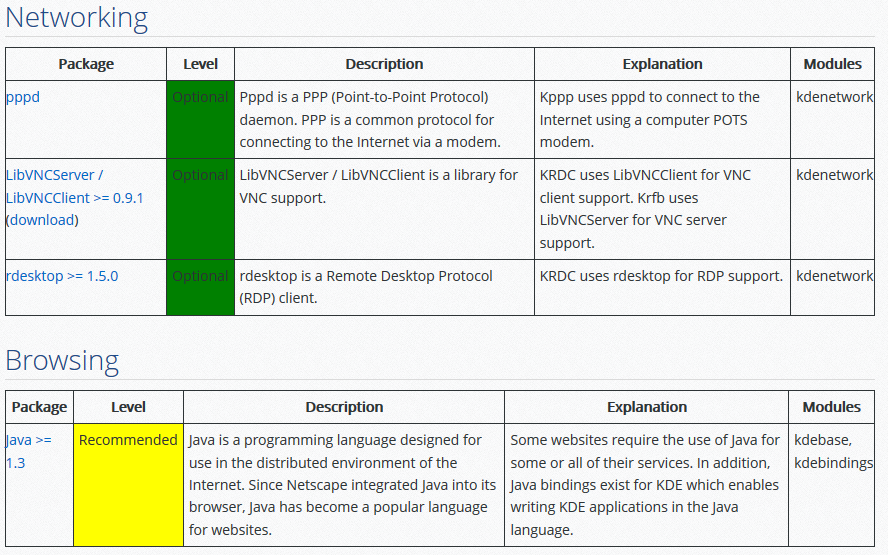
\includegraphics[width=\columnwidth]{images/KDE_Net_B.png}
\caption{Networking und Browsing\cite{6}}
\end{figure}
%network games req optional Contact
Das Bild zeigt zwei Tabellen die der Quelle, der KDE
Website entnommen wurden\cite{6}.
%Quelle:https://techbase.kde.org/Schedules/KDE4/4.4_Requirements
Die Tabellen haben jeweils 5 Spalten. Die erste Spalte enthält den Namen des
Packages das unter Umständen benötigt wird. Die zweite Spalte enthält das Level,
also wie stark die Funktion abhängig von dem Requirement ist, unterteilt in
Required, Recommended und Optional. Die dritte Spalte enthält eine Beschreibung
was dieses Package enthält und die vierte Spalte eine Erklärung warum dieses
Requirement für die Funktion nötig ist. In der fünften und letzten Spalte ist
festgehalten zu welchem Modul das Package gehört.

\subsection{Fazit}
Abschließend kann ich zum Requirements Engineering bei KDE sagen, dass das
Vorgehen mir schon zu Beginn meiner Nachforschung ähnlich zu dem vorkam, was ich
über das Vorgehen bei der Arbeit an Linux selbst erfahren habe. Das Aufteilen
der Aufgaben an verschiedene Personen die dann zuständig sind und stark dafür
verantwortlich die Requirements zu fassen bzw. zu bestimmen. Dies hat sich
auch beim Abschluss meiner Nachforschung bestätigt, weshalb ich dieses Vorgehen
im obrigen Teil auch wiedergegeben habe. Dieses Vorgehen ist für gewöhnliche
Projekte eher untypisch und unterschiedet sich auch von den klassischen Methoden
die in der Vorlesung aufgeführt wurden. %Für Open Source Projekte ist zwar ein
%anderes Vorgehen erfordlich aber es hätte bestimmt auch eine andere Möglichkeit
%gegeben.
Wobei dazuzusagen ist, dass KDE ein Open Source Projekt ist und deswegen eine
andere Vorgehensweise erfordert und es genauso seine Berechtigung hat, den KDE
und Linux sind beide erfolgreiche Projekte.
%untypisches requirement Engineering kein normales
%aufsteleln typisch linux / Open Source?
%two Bilder ..
%Linux typisch guru
\begin{thebibliography}{x}
   \bibitem[1]{1}'https://de.kde.org/'
   \bibitem[2]{2}'http://www.enzyklopaedie-der-wirtschaftsinformatik.de/lexikon/is-management/Systementwicklung/Hauptaktivitaten-der-Systementwicklung/Problemanalyse-/Requirements-Engineering/index.html'
   \bibitem[3]{3}'https://techbase.kde.org/Development/Software\_Engineering\_Framework\#Requirements\_Gathering'
   \bibitem[4]{4}'https://docs.kde.org/index.php?language=de\&package=kdemultimedia'
   \bibitem[5]{5}'https://techbase.kde.org/Schedules/Applications/15.12\_Feature\_Plan'
   \bibitem[6]{6}'https://techbase.kde.org/Schedules/KDE4/4.4\_Requirements'
\end{thebibliography}



\documentclass[10pt,a4paper,twocolumn]{article}
\usepackage[utf8]{inputenc}
\usepackage[ngerman]{babel}
\setlength{\parindent}{0cm}
\usepackage[colorlinks=true, urlcolor=black]{hyperref}
\usepackage{graphicx}
\begin{document}
	
\section{Prozesse}
Dieses Kapitel befasst sich mit der Betrachtung der KDE Entwicklungs- und Organisationsprozesse. Nach der Beleuchtung des sogenannten Application Lifecycle, also wie Neuentwicklungen gehandhabt werden, betrachten wir das Projektmanagement, sowie die Kommunikation und Arbeit der verschiedenen Teams.

\subsection{KDE Application Lifecycle \cite{ApplLife}} 
\begin{figure}[h]
	\centering
	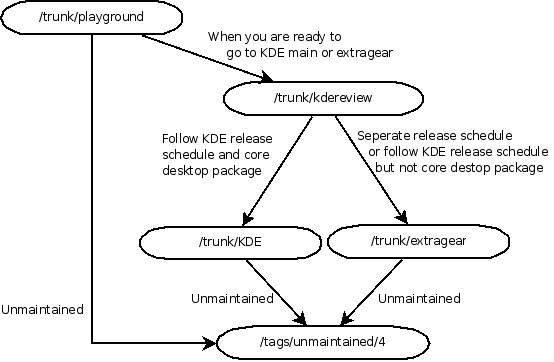
\includegraphics[width=\columnwidth]{images/KDE_application_lifecycle.png}
	\caption{KDE Applicatuion Lifecycle \cite{ApplLife}}
	\label{fig:kde_applLife}
\end{figure}
In Abbildung \ref{fig:kde_applLife} ist schön zu sehen, wie der Lebenszyklus einer KDE-Anwendung aussieht, welche auf Eigeninitiative eines Entwicklers implementiert wurde.\\
Zu Beginn kann lokal mit der KDE-Entwicklungsumgebung programmiert werden. Möchte man seine Anwendung in einem der kommenden Releases enthalten haben, muss man den entsprechenden Code samt Dokumentationspapier ins Subversion Repository committen (Wird momentan komplett auf Git umgestellt). Speziell dafür gibt es die sogenannte Spielwiese (/trunk/playground), auf welcher ohne jede Einschränkung programmiert werden darf.\\
Sollte sich der Entwickler dazu entscheiden, die neue Anwendung gerne zusammen mit dem Release Plan von KDE zu veröffentlichen, wird das Projekt auf die nächste Stufe geschoben, dem sogenannten KDE Review.\\
Dieser Schritt stößt ein zweiwöchiges Review innerhalb der KDE Community an. Führte diese zweiwöchige Phase zu keinerlei Änderungswünschen, hat der Entwickler die Erlaubnis, seine Neuentwicklkung ins produktive KDE zu übernehmen. Je nachdem, ob man dem festen Release Plan von KDE folgen oder darin frei sein möchte, wird das entsprechende Verzeichnis gewählt.\\
Eine letzte Hürde für den KDE Release Plan ist die Zustimmung des entsprechenden Modulkoordinators.\\
Sofern im Review-Status erst noch Änderungen und Bugfixes anstehen, darf je nach Verfügbarkeit des Entwicklers das Projekt bis zur Fehlerbehebung im Review-Status bleiben oder muss auf die Spielwiese zurückgesetzt werden. Dadurch befinden sich nur diejenigen Projekte im Review-Status, an welchen noch regelmäßig weiterentwickelt wird und keine Altlast-Projekte.
\cite{ApplLife}

\subsection{KDE Release Team \cite{KDEReleaseTeam}}
Das KDE Release Team ist zuständig für die Koordination aller offiziellen KDE Releases. Dies beinhaltet unter Anderem die Erstellung eines Zeitplans, die Einplanung von Marketingaufwänden, als auch die Kontrolle zur Einhaltung von Deadlines oder Code-Restriktionen.\\
\begin{figure}[h]
	\centering
	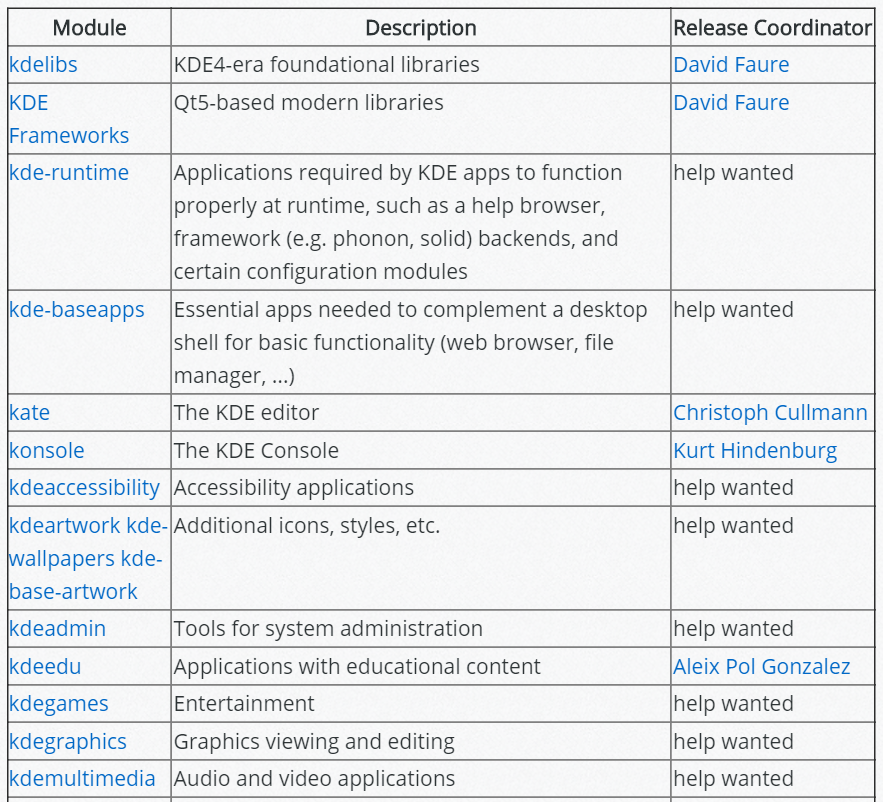
\includegraphics[width=\columnwidth]{images/KDE_module_coordinators.png}
	\caption{Auszug der Liste von KDE-Modulkoordinatoren \cite{KDEReleaseTeam}}
	\label{fig:kde_moduleKoord}
\end{figure}
Der Entscheidungsfindungsprozess soll laut offizieller KDE-Richtlinie öffentlich sein und es können Anregungen sowie Wünsche von allen Seiten eingereicht werden.\\
Personell setzt sich das Release Team aus den einzelnen Modulkoordinatoren der verschiedenen KDE-Module, sowie dem Marketing Team und diversen Personen für die Verwaltung der Planungen zusammen.\\
Die Kommunikation erfolgt wie üblich über Mailing-Listen oder direkte E-Mails. \cite{KDEReleaseTeam} \\ \\
Im Auszug aus Abbildung \ref{fig:kde_moduleKoord} ist deutlich zu sehen, dass nicht einmal die Hälfte der Module bislang einen fixen Modulkoordinator zugewiesen haben. Genau genommen existieren gerade einmal für 9 der 23 KDE-Module solche Personen.\\
Selbst vermeintlich wichtige Posten wie für die Systemadministration sind nicht offiziell besetzt, was sich als großer Schwachpunkt der aktuellen Projekt-Organisation herausstellen könnte.\\ \\
Die Aufgabe des gesamten Release Teams besteht erstens darin, sicherzustellen, dass sich die Neuentwicklungen in einem auslieferbaren Zustand befinden.\\
Die zweite Kernkompetenz liegt darin, neue Features für zukünftige Releases zu sammeln und zu organisieren. Dabei entscheidet das Release Team auch, welche Features wirklich umgesetzt oder verworfen werden. \cite{KDEReleaseTeam} \\ \\
Zusammenfassend lässt sich sagen, dass das Release Team eine zentrale Instanz für die Organisation der Projekte darstellt. Es beherbergt die Überwachung geplanter Entwicklungen, als auch die Entscheidungskraft für künftige Entwicklungen.

\subsection{Code Reviews \cite{KDECodeReview}}
Dieses Kapitel befasst sich mit den Code-Reviews...
\begin{center}
	\textbf{{\LARGE TODO}}
\end{center}

\subsection{KDE Release Schedule - Beispiel Plasma 5 \cite{KDEReleaseSchedulePlasma5}}
Dieses Kapitel zeigt einen beispielhaften Release Plan von Plasma 5 (siehe Abbildung \ref{fig:kde_schedulePlasma5}). Der Zeitplan ist das Ergebnis des eben erläuterten Release Teams.
\begin{figure}[h]
	\centering
	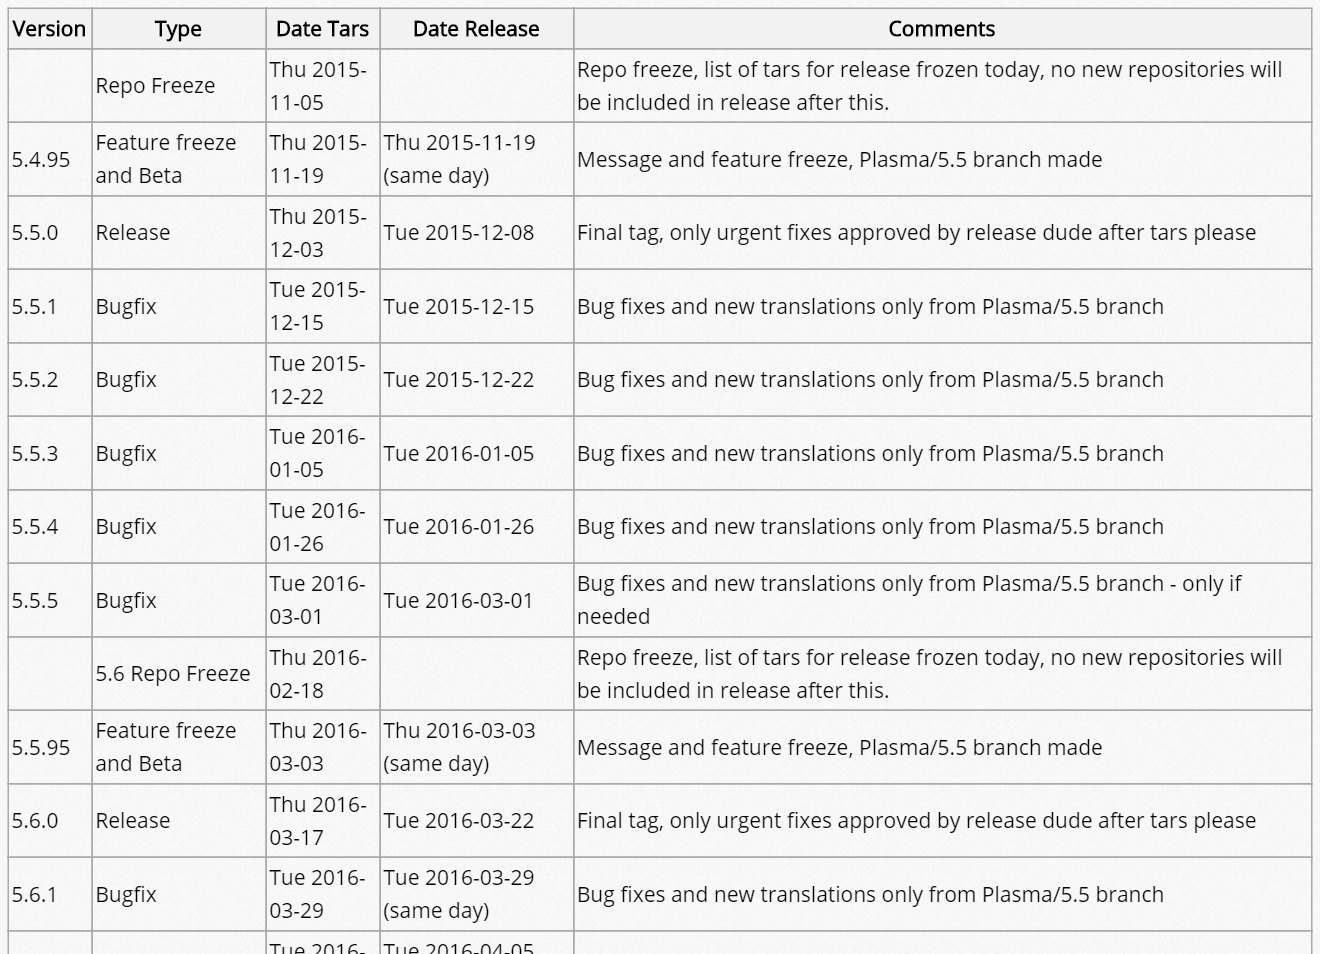
\includegraphics[width=\columnwidth]{images/KDE_schedule_plasma5.png}
	\caption{Auszug des Release Schedule von KDE Plasma 5 \cite{KDEReleaseSchedulePlasma5}}
	\label{fig:kde_schedulePlasma5}
\end{figure}
\begin{center}
	\textbf{{\LARGE TODO}}
\end{center}

% Literaturverzeichnis (quellen.bib)
\bibliography{quellen}{}
\bibliographystyle{alpha}
% Abbildungsverzeichnis
\listoffigures

\end{document}
%\documentclass[10pt,a4paper,twocolumn]{article}
%\usepackage[utf8]{inputenc}
%\usepackage[ngerman]{babel}
%\setlength{\parindent}{0cm}
%\usepackage[colorlinks=true, urlcolor=black]{hyperref}
%\usepackage{graphicx}
%\begin{document}
	
% TODO: KDE Plasma detailierter Beschreiben
% TODO: Ein Teil / ein Subproject detailliert Beschreiben (Analyse mit Tool [cppdepend?])
	
\section{KDE Architecture}
Im Folgenden wird nun die Architektur der vom Team des KDE Projekts entwickelten KDE Software Compilation (KDE SC) vorgestellt. Der wohl bekannteste Teil der KDE Software Compilation ist die Desktop Umgebung KDE Plasma. Dazu kommt eine große Anzahl an Anwendungen die KDE Applications. Diese werden vor allem in Verbindung mit KDE Plasma genutzt können aber auch unabhängig davon verwendet werden. Der dritte Bestandteil der KDE Software Compilation heißt KDE Frameworks und stellt eine Sammlung von Bibliotheken dar. Diese enthalten häufig benötigte Funktionen und machen es somit einfacher KDE Software zu entwickeln. Außerdem wird so das ständige neu entwickeln grundlegender Funktionen verhindert. Wichtig ist in diesem Zusammenhang auch die Qt Library die zwar nicht direkt zum KDE Projekt gehört aber eng mit dem KDE Projekt verbunden ist da Qt als Basis für die Entwicklung verwendet wird.
Qt (http://www.qt.io/) ist im wesentlichen eine C++-Klassenbibliothek für die plattformübergreifende Programmierung grafischer Benutzeroberflächen die viele für die Entwicklung hilfreiche Funktionen bietet.
%\url{https://en.wikipedia.org/wiki/Qt_(software)}
%\url{http://www.qt.io/}
Auf Anwenderebene sind also die KDE Applications und KDE Plasma die auf die KDE Framworks und Qt aufbauen wie auch in Abbildung \ref{fig:kde_overview} dargestellt.
\begin{figure}[h]
\centering
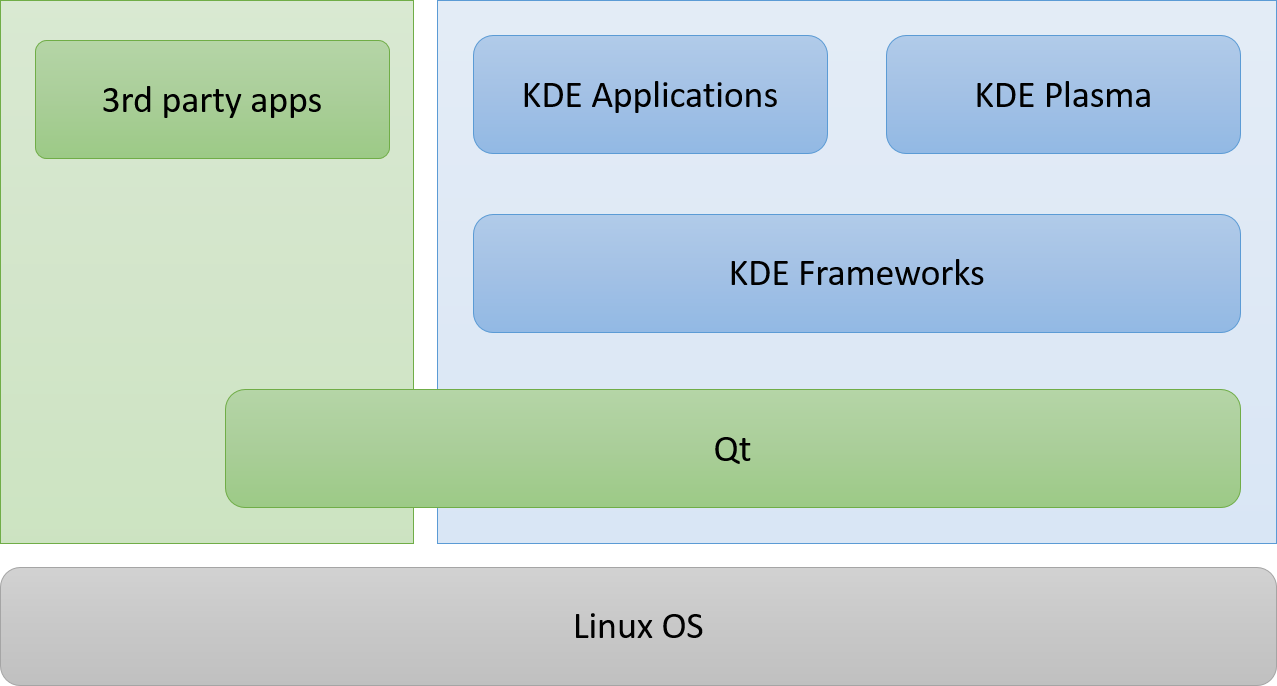
\includegraphics[width=0.9\columnwidth]{images/KDE_Aufbau.png}
\caption{KDE Übersicht}
\label{fig:kde_overview}
\end{figure}

\subsection{KDE Frameworks 5}
Das Ziel des unter der LGPL stehenden und vor allem in C++ und C entwickelten KDE Frameworks ist die Modularisierung. Aufbauend auf das als Basis genutzte Qt 5 stellt das aktuelle KDE Frameworks 5 grundlegende und für viele Anwendungsfälle nützliche Funktionen wie z.B. extra UI Elemente, Rechtschreibprüfung, usw. zu Verfügung. KDE Frameworks stellt somit durch seine verschiedenen Bibliotheken die Basis für KDE Plasma und KDE Applications dar und vereinfacht die Entwicklung, da auf erprobte Implementierungen zurückgriffen werden kann und unnötiges für jede Software neu entwickeln verhindert wird. Das KDE Frameworks 5 besteht dazu aus rund 60 einzelnen Bibliotheken mit verschiedenen Abhängigkeiten untereinander die möglichst Plattform unabhängig gehalten sind und versuchen so wenig wie möglich zusätzliche Abhängigkeiten zu verursachen. Für eine bessere Übersicht welche Abhängigkeiten existieren erfolgt dabei eine Einteilung ist nach "'Tier"' und "'Categorie"' die im Folgenden auch noch detaillierter vorgestellt wird. Abbildung \ref{fig:kde_frameworks} gibt einen groben Überblick für die Bestandteile der KDE Frameworks 5 und zu welchen "'Tier"' sie gehören.
%\url{https://dot.kde.org/2013/09/25/frameworks-5}
%https://www.kde.org/ https://dot.kde.org/ http://api.kde.org/

%\url{https://dot.kde.org/2014/01/07/frameworks-5-tech-preview}
%\url{https://dot.kde.org/sites/dot.kde.org/files/kf5_big_0.png}
\begin{figure}[h]
	\centering
	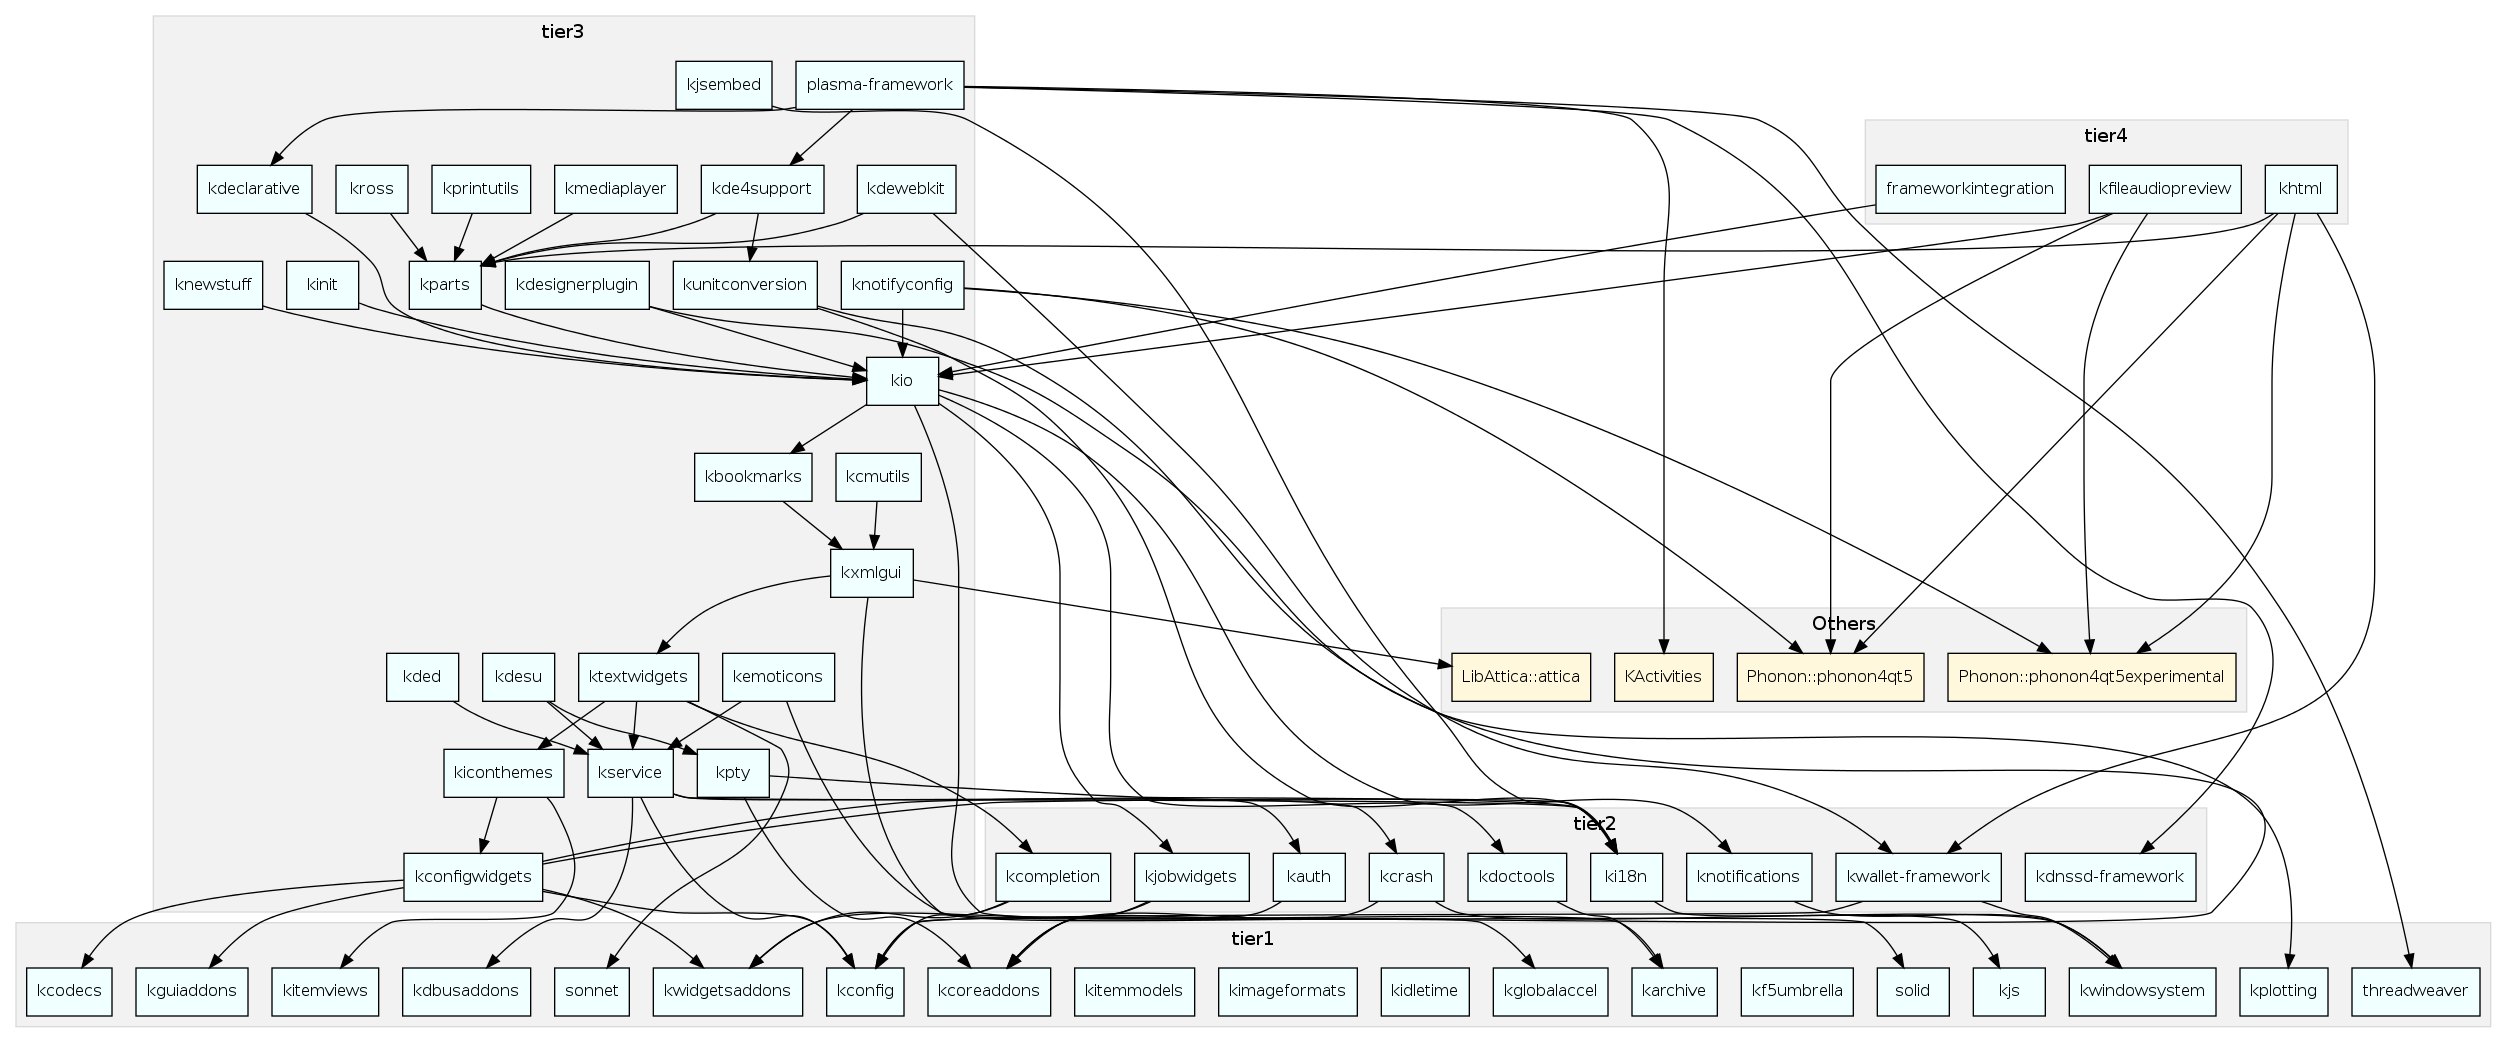
\includegraphics[width=\columnwidth]{images/kf5_big_0.png}
	\caption{KDE Frameworks}
	\label{fig:kde_frameworks}
\end{figure}

Ziel der Aufteilung in viele einzelne in KDE Frameworks gebündelte Bibliotheken ist dabei dass es leichter möglich wird nur auf Teile der KDE Frameworks aufzubauen.
Die vielen einzelnen Bibliotheken von denen immer nur die benötigen verwendet werden ist dabei eine noch recht neue für die Architektur der Software sehr wichtige Entwicklung die erst mit KDE Frameworks 5 im Dezember 2013 eingeführt wurde. KDE Frameworks in Version 4 trug noch den Namen KDE Platfrom baute noch auf Qt 4 und war im Prinzip nur eine einzige große KDElibs Library wie sie schon in den Versionen davor existierte.
%\url{https://en.wikipedia.org/wiki/File:Evolution_and_development_of_KDE_software.svg}
\begin{figure}[h]
\centering
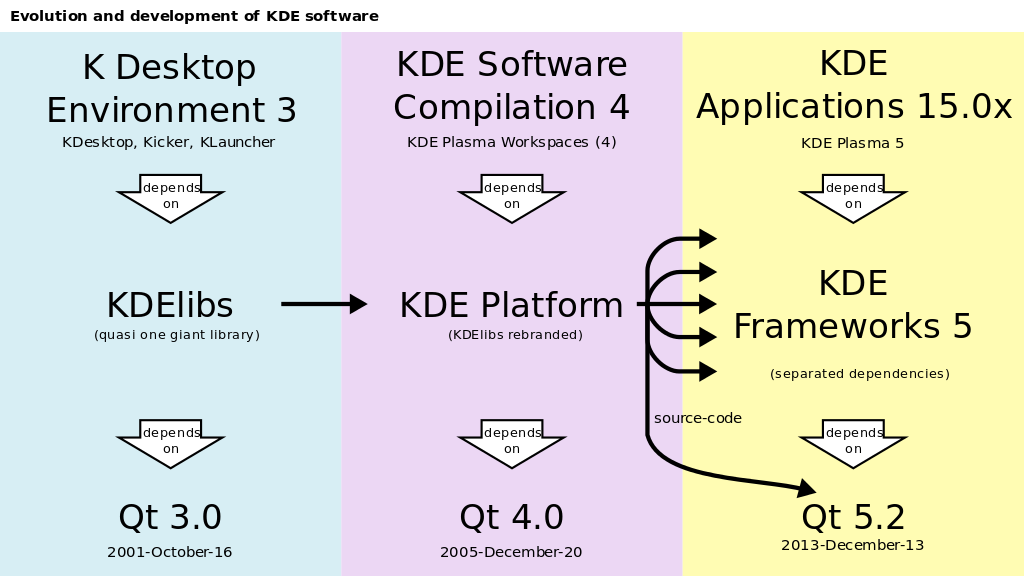
\includegraphics[width=\columnwidth]{images/Evolution_and_development_of_KDE_software}
\caption{KDE Frameworks}
\label{fig:Evolution_and_development_of_KDE_software}
\end{figure}

Große umbauten auf KDE Frameworks Ebene wie z.B. von Version 4 auf 5 beeinflussen allerdings alle darauf aufbauende Software weshalb verschiedene KDE Frameworks Versionen parallel von verschieden Anwendungen genutzt werden können, so dass Anwendungen die darauf aufbauen in Ruhe beim erscheinen einer neuen Version auf diese portiert werden können. Major Releases (Versionsnummer X.0) brechen dabei die Abwärtskompatibilität und steigen auch auf die nächste große Qt Version um. Minor Veröffentlichungen (X.1, X.2, ...) hingegen garanteiren Source und Binär Kompatibilität und sind meist kleine Weiterentwicklungen, Verbesserungen und vor allem Fehlerkorrekturen.

%https://www.kde.org/developerplatform/
Bekannte Frameworks aus den KDE Framworks 5 sind z.B. Sonnet eine Rechtschreib- und Grammatikprüfung, KHTML eine HTML und JS Library, Solid eine Hardware und Network Abstraktion und Phonon ein Multimedia Framework. Eine Vollständige Liste ist in der online API Dokumentation zu finden.

Die KDE Frameworks 5 haben dabei eine klare Dependency Struktur die in "'Categorie"' und "'Tier"' einteilt. Dies hilft den Überblick zu behalten welche Abhängigkeiten der Einsatz eines bestimmten Framework mit sich bringt. In der online API Dokumentation ist deshalb auch eine Zuordnung der Farmeworks zu den Tiers verfügbar.
%\url{https://dot.kde.org/2013/09/25/frameworks-5}
%\url{http://api.kde.org/frameworks-api/frameworks5-apidocs/}

Die Einteilung "'Categories"' bezieht sich dabei auf Laufzeit-Abhängigkeiten:
\begin{itemize}
\setlength\itemsep{0em}
\item Functional: Auf Qt aufbauend und ohne weitere Laufzeit-Abhängigkeiten z.B. KArchive, KPlotting, Threadweaver, KConfig, KCoreAddons

\item Integration: Mit optionalen Laufzeit-Abhängigkeiten für Integration bzw. Kompatibilität mit Betriebssystem/Plattform darunter z.B. Sonnet, Solid

\item Solutions: Haben gewollt Laufzeit-Abhängigkeiten um sich damit ergebende Vorteile nutzen zu können z.B. KIO, KService
\end{itemize}

Die Einteilung in "'Tiers"' bezieht sich auf Compile-Zeit Abhängigkeiten:
\begin{itemize}
\setlength\itemsep{0em}
\item Tier 1: Keine Abhängigkeiten innerhalb KDE Frameworks, nur Ot und andere kleine Abhänglichkeiten  checkerso dass eine einfach Verwendung in einem Qt Projekt möglich ist. 

\item Tier 2: Dürfen auf Tier 1 Frameworks aufbauen haben aber weiterhin einfach zu verwaltende Abhängigkeiten.

\item Tier 3: Dürfen auf Tier 3 Farmworks genauso wie Tier 2 und Tier 1 Frameworks aufbauen und haben somit oft schon komplexere Abhängigkeiten.

\item Tier 4: Für Anwendungsentwickler unwichtig vor allem Frameworks zur Integration. 
\end{itemize}

Jedes Framework lässt sich somit klar einordnen. Außerdem gibt es eine vom KDE Projekt erstelle Tier/Categorie Matrix (siehe Abbildung \ref{fig:kde_matrix}) die verschieden sich damit ergebenden Kombinationen und Abhängigkeiten Zeigt.

%\url{https://dot.kde.org/sites/dot.kde.org/files/kf5_no_tier4_big.png}
\begin{figure}[h]
	\centering
	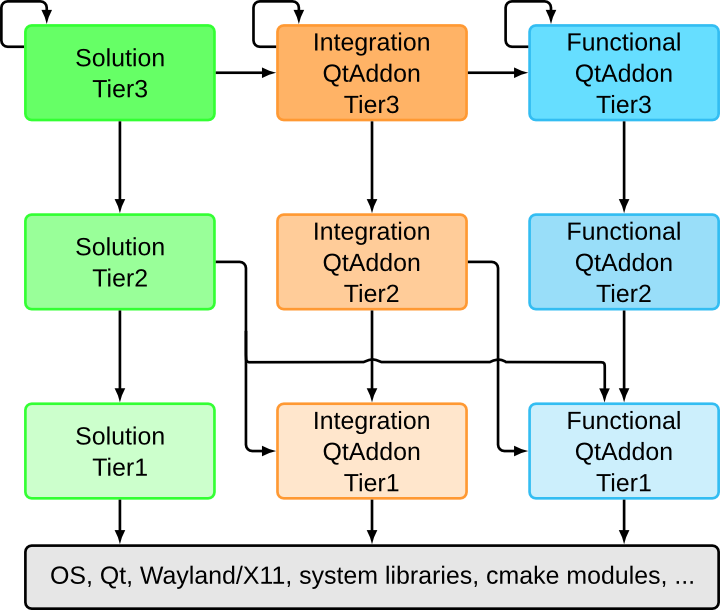
\includegraphics[width=0.9\columnwidth]{images/kf5_no_tier4_big.png}
	\caption{KDE Tier/Categorie Matrix}
	\label{fig:kde_matrix}
\end{figure}

\subsection{KDE Plasma 5}
KDE Plasma 5 stellt die bekannte für Linuxsysteme entwickelten Arbeitsplatzumgebung des KDE Projekts dar. Aufbauend auf Qt 5 und KDE Frameworks 5 findet die Entwicklung vor allem mit C++ und QML statt. 

\url{https://en.wikipedia.org/wiki/KDE_Plasma_5}
\url{http://www.heise.de/open/artikel/Plasma-5-Der-KDE-Desktop-in-neuem-Glanz-2260451.html}

// TODO: Details zur Architektur (Mit Tool wenn es sich anbietet sonst für ein einfacheres Beispiel aus dem nächsten Abschnitt)

\subsection{KDE Applications 15.12}
Viele einzelne Anwendungen die zum KDE Projekt gehören werden unter den KDE Applications zusammengefasst. Das KDE Projekt Teil die über hundert Anwendungen deshalb zur besseren Übersicht deswegen die die Kategorien Development, Education, Games, Graphics, Internet, Multimedia, Office, System und Utilities ein. Die verschieden Anwendungen der KDE Applications bauen wie KDE Plasma auf Qt und KDE Frameworks auf. Davon Abgesehen sind die einzelnen Anwendungen aber relativ unabhängig vom gesamt Projekt gehalten weshalb auch die Architektur der einzelnen Programme betreffende Entscheidungen variieren. 

// TODO: Eventuell ein Beispiel detaillierter

\url{https://en.wikipedia.org/wiki/KDE_Applications}

%\end{document}

\section{Conclusions}
This paragraph will end the body of this sample document. 
Remember that you might still have Acknowledgments or
Appendices; brief samples of these
follow.  There is still the Bibliography to deal with; and
we will make a disclaimer about that here: with the exception
of the reference to the \LaTeX\ book, the citations in
this paper are to articles which have nothing to
do with the present subject and are used as
examples only.
%\end{document}  % This is where a 'short' article might terminate



%
% The following two commands are all you need in the
% initial runs of your .tex file to
% produce the bibliography for the citations in your paper.
\bibliographystyle{abbrv}
\bibliography{quellen}  % sigproc.bib is the name of the Bibliography in this case
% You must have a proquper ".bib" file
%  and remember to run:
% latex bibtex latex latex
% to resolve all references
%
% ACM needs 'a single self-contained file'!
%
%APPENDICES are optional
%\balancecolumns

\end{document}
